\section{Tool Implementation}\label{sec:tooling}

\ctVerif is an open-source implementation of the constant-time verifier we
described earlier in \secref{body}. \figref{ct-verif-flow} illustrates the
tool flow from top to bottom. To prove constant-time security, a C function is
instantiated in a proof harness that categorizes inputs and outputs as public/secret. Then,
the function and its harness are compiled down to \codetext{llvm} bitcode. The
bitcodes are linked together and converted to \emph{Boogie Programming
Language} (\codetext{.bpl}). Compilation down to \codetext{.bpl} is automated
through \emph{SMACK}~\cite{smack}, but it is possible to customize the flow if
needed and only rely on the the \codetext{bitcode}-to-\codetext{bpl} conversion
of SMACK.

The linked \codetext{bpl} files are then fed to \emph{BAM! BAM! Boogieman} which
performs the key task of generating the self-product (c.f. \secref{body}), and
finally the self-product---which contains assertions and assumptions---is
given to \emph{Boogie}~\cite{boogie} to verify assertion safety.


\begin{figure}[h]
    \centering
    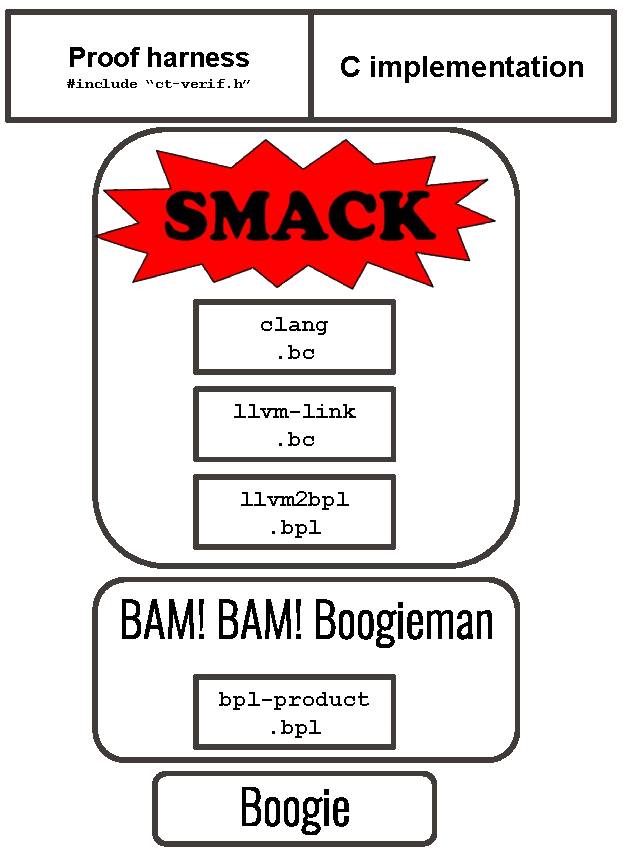
\includegraphics[height=0.4\textheight]{figs/ct-verif-flow.pdf}
    \caption{\ctVerif tool flow}
    \label{fig:ct-verif-flow}
\end{figure}




To ensure the tool works as advertised, we first tried proving/disproving
small examples with obvious answers before reproducing the
results reported in the paper~\cite{almeida}.


\subsection{Handling toy programs}

We started by disproving constant-timeness of the code given in \figref{example}.
\ctVerif correctly identifies this code as unsafe (i.e., not constant-time).
The test harness for this examples is a simple wrapper that declares all inputs
as public except \codetext{l\_idx}.

\begin{figure}[h]
    \centering\resizebox{0.7\columnwidth}{!}{\lstinputlisting[language=C]{code/example_wrapper.c}}
    \caption{Proof harness for sub-array copy in \figref{example}.}
    \label{fig:example_wrapper}
\end{figure}

A more interesting example is the slightly unusual \codetext{vector\_add}
function in \figref{vector_add}. Notice how by declaring \codetext{a[N - 1]} as
a public input we make the code constant time. \ctVerif also successfully
identifies this code as constant time. Now if we remove the public input
declaration on line 10, then the code will no longer be constant time because the
for loop will leak the length of arrays and \ctVerif also correctly marks the
program as non-constant time.

\begin{figure}[h]
    \centering\resizebox{0.7\columnwidth}{!}{\lstinputlisting[language=C]{code/vector_add.c}}
    \caption{A slightly unusual vector addition.}
    \label{fig:vector_add}
\end{figure}


\subsection{Reproducing results}


We set out to reproduce all the results in the paper, however, we ended up
only verifying some of them. There were two reasons:
\begin{enumerate}
    \item Functions reported as constant-time in the paper could not be proven
    to be constant-time using \ctVerif;
    \item The reported functions could not be found in the \ctVerif repository,
    or their build procedures were broken/incomplete.
\end{enumerate}

\subsubsection{\codetext{tea}}
\codetext{tea} is a tiny encryption algorithm that consists of about 20 lines
of code. We successfully verified \codetext{tea} to be constant-time.



\subsection{\codetext{libfixedpointfixedtime}} \codetext{libfixedpointfixedtime}
is a library that implements a large variety of fixed-point arithmetic
operations in constant-time. The paper only reports constant-timeness for 10
functions in the library, but we managed to verify an additional 24 functions using \ctVerif
that were not reported in the paper. These additional functions are:
\codetext{fix\_is\_neg},
\codetext{fix\_is\_nan},
\codetext{fix\_is\_inf\_pos},
\codetext{fix\_is\_inf\_neg},
\codetext{fix\_eq},
\codetext{fix\_eq\_nan},
\codetext{fix\_ne},
\codetext{fix\_cmp},
\codetext{fix\_le},
\codetext{fix\_ge},
\codetext{fix\_lt},
\codetext{fix\_gt},
\codetext{fix\_neg},
\codetext{fix\_abs},
\codetext{fix\_add},
\codetext{fix\_sub},
\codetext{fix\_mul},
\codetext{fix\_div},
\codetext{fix\_floor},
\codetext{fix\_ceil},
\codetext{fix\_ln},
\codetext{fix\_log2},
\codetext{fix\_log10},
\codetext{fix\_convert\_from\_int64},
\codetext{fix\_convert\_to\_int64},
\codetext{fix\_round\_up\_int64},
\codetext{fix\_ceil64},
\codetext{fix\_floor64},
\codetext{fix\_sin},
\codetext{fix\_cos},
\codetext{fix\_tan},
\codetext{fix\_exp},
\codetext{fix\_sqrt},
\codetext{fix\_pow}.

\subsubsection{\codetext{curve25519-donna}} We successfully re-verified the C
implementation of the \codetext{curve25519-donna} elliptic curve. This function
was the hardest among all and took the longest time to prove (about 7 minutes).


\subsubsection{\codetext{libsodium}} \codetext{libsodium} is an easy-to-use
encryption library. We attempted to verify 4 functions here (\codetext{chacha20,
salsa20, sha256, sha512}). We used the Makefiles
provided by \ctVerif which isolate the C files used by each function (i.e., the
whole library is not compiled to \codetext{llvm} bitcode). We successfully
reproduced the paper results by verifying constant-timeness of
\codetext{chacha20} and \codetext{salsa20}, but failed prove it for
\codetext{sha256} and \codetext{sha512} (unlike what the paper claims).


Upon inspecting the C implementation of \codetext{sha256} and \codetext{sha512}
we couldn't identify exactly why these two functions are not constant-time.
This implored us look for other methods of asserting constant-timeness which
we will follows up on in \secref{discussion}.



\subsection{Scalability of \ctVerif}

To evaluate the scalability of this tool we first tried to verify
constant-timeness of function \codetext{s2n\_verify\_cbc} from Amazon's
\codetext{libs2n} library. The test harness for this function is included as one of the
examples in the \ctVerif repository but it had a simple bug where the test
harness was calling itself instead of the \codetext{s2n\_verify\_cbc} function.
However, there was no build script for this specific function and we had to modify the
\codetext{Makefile}s in the \codetext{libs2n} library to generate
\codetext{llvm} bitcode instead of a binary. We then manually linked the bitcode
library with the test harness and invoked \codetext{llvm2bpl} pass---provided by
SMACK---and fed the generated \codetext{.bpl} files to BAM! BAM! Boogie to
generate the program product. Unfortunately. \codetext{llvml2pl} resulted in
many warnings regarding memory safety and self-product program generation failed
to due an resolved reference.


In another attempt, we compiled the OpenSSL library down to \codetext{llvm}
bitcode to verify the SHA-1 function. Transformation from bitcode to bpl
resulted in over 70GiB of memory usage and did not terminate after 30 minutes.


Unlike the functions verified in the paper, these two functions are not
isolated and the bitcode given to \ctVerif contains unused code. It seems like
SMACK transforms the whole program irrespective of the target function. This
approach limits the usability of \ctVerif since verifications requires a good
understanding of the underlying library structure to be able to isolate the used
code.

